\documentclass[12pt]{article}

\usepackage{amsmath}
\usepackage{amssymb}
\usepackage{bm}
\usepackage{enumerate}
\usepackage{fancyvrb}
\usepackage[top=1in, bottom=1in, left=1in, right=1in]{geometry}
\usepackage{hyperref}
\usepackage{placeins}
\usepackage{tikz}
\usepackage{tikzsymbols}
\usepackage{todonotes}

\usetikzlibrary{positioning,calc}

\title{10-703 Deep RL and Controls\\
  Homework 1\\
  Spring 2017\\
}

\date{February 1, 2017\\
  \hspace{1cm}\\
Due February 17, 2017}

\begin{document}

\maketitle

\section*{Instructions}

You have 15 days from the release of the assignment until it is
due. Refer to gradescope for the exact time due.

You may work with a partner on this assignment. Only one person should
submit the writeup and code on gradescope. Make sure you mark your
partner as a collaborator on gradescope and that both names are listed
in the writeup.

Writeups should be submitted as PDF.

% \section*{Problem 1}

% \todo[inline]{Show that Bellman backup converges to a fixed point with
% max version of equation.}

\section*{Problem 1}
\label{sec:p1}

% \todo[inline]{Ask them to set up as linear system in numpy and solve.}


Consider an environment in which our agent requires caffeine to
function\footnote{If it helps you can think of the agent as a graduate
  student.}. Because caffeine is so important to our agent, we would
like the agent to find a policy that will always lead it to
the shortest path to coffee. Once the agent reaches coffee, it
will stick around and enjoy it.

In order to apply optimal control techniques such as value
iteration and policy iteration, we first need to model this
scenario as an MDP. Recall that an MDP is defined as tuple
$(S, A, P, R, \gamma)$, where:
\begin{description}
\item[$S$:] The (finite) set of all possible states.
\item[$A$:] The (finite) set of all possible actions.
\item[$P$:] The transition function $P: S \times S \times A \to [0, 1]$, 
  which maps $(s', s, a)$ to $P(s'|s, a)$, i.e., 
  the probability of transitioning to state $s'\in S$ when taking action
  $a\in A$ in state $s\in S$. 
  Note that $\sum _{s' \in S} P(s' | s, a) = 1$ for all 
  $s \in S, a \in A$.
\item[$R$:] The reward function $R : S \times A \times S \to \mathbb R$,
which maps $(s, a, s')$ to $R(s, a, s')$, i.e., 
the reward obtained when taking action $a \in A$ in state $s \in S$ and 
arriving at state $s' \in S$.
\item[$\gamma$:] The discount factor, which controls how important are 
  rewards in the future. We have $\gamma \in [0, 1)$, where smaller values 
  mean more discounting for future rewards.
\end{description}

In order to encode this problem as an MDP, we need to define each of
the components of the tuple for our particular problem. 
Note that there may be many different possible encodings.

For the questions, in this section, consider the instance shown in
Figure~\ref{fig:prob1_shortest_path_domain}. In the figure, the agent
is at $(1,1)$, but it can start at any of
the grid cells. The goal, displayed as a coffee cup, is
located at $(6,6)$. The agent is able to move one square up, down,
left and right (deterministically). Walls are represented by thick black
lines. The agent cannot move through walls. All actions are available in
all states. If the agent attempts to move through a wall, 
it will remain in the same state.

When the agent reaches the coffee cup, the episode ends. Another way to
think of this, is that every action in the coffee cup state, keeps the
agent in the coffee cup state.

\begin{figure}
  \centering
  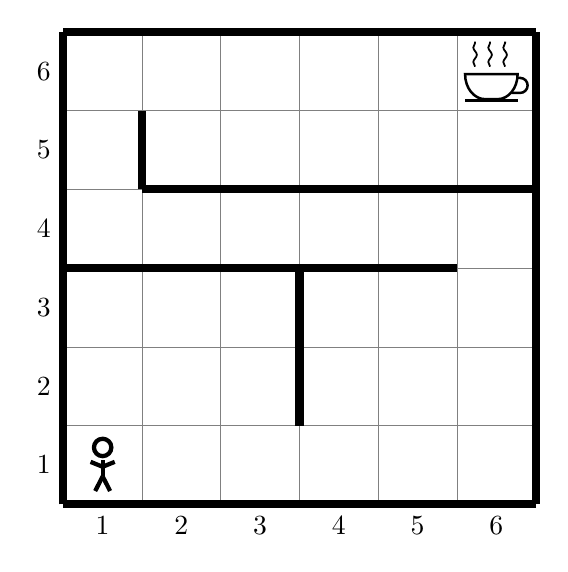
\begin{tikzpicture}
    % draw the grid and label the edges
    \draw[step=1cm,gray,very thin] (0,0) grid (6,6);
    \foreach \x in {1, ..., 6}
      \draw (\x cm - .5cm, 1pt) -- (\x cm - .5cm, -1pt)
      node[anchor=north] {$\x$};
      \foreach \y in {1, ..., 6}
      \draw (1pt,\y cm - .5cm) -- (-1pt, \y cm - .5cm)
      node[anchor=east] {$\y$};

      % add the agent and the goal
      \node (agent) at (.5cm, .5cm) {\Strichmaxerl[3]};
      \node (goal) at (5.5cm, 5.5cm) {\Coffeecup[3]};

      % Add some obstacles
      \draw[line width=3pt] (0cm, 3cm) -- (5cm, 3cm);
      \draw[line width=3pt] (3cm, 3cm) -- (3cm, 1cm);

      \draw[line width=3pt] (1cm, 4cm) -- (6cm, 4cm);
      \draw[line width=3pt] (1cm, 4cm) -- (1cm, 5cm);

      % border walls
      \draw[line width=3pt] (0cm, 0cm) -- (0cm, 6cm);
      \draw[line width=3pt] (0cm, 0cm) -- (6cm, 0cm);
      \draw[line width=3pt] (6cm, 6cm) -- (0cm, 6cm);
      \draw[line width=3pt] (6cm, 6cm) -- (6cm, 0cm);

  \end{tikzpicture}
  \caption{\label{fig:prob1_shortest_path_domain} A particular
    instance of the shortest path problem. The goal is for the agent
    currently located in state $(1,1)$ to have a policy that always
    leads it on the shortest path to the coffee in state $(6,6)$.}
\end{figure}

\subsection*{Part a (10pt)}

For this section, assume we are modeling the MDP as an infinite
horizon MDP. The coffee cup is still an absorbing state.

Using the above problem description answer the following questions:

\begin{enumerate}[a)]
\item  How many states are in this MDP? (i.e. what is $|S|$).
\item How many actions are in this MDP? (i.e. what is $|A|$).
\item What is the dimensionality of the transition function $P$?
\item Fill in the probabilities for the transition function $P$.\\
  \begin{center}
    \begin{tabular}{|l|l|c|c|c|c|c|}\hline
      \multicolumn{2}{|c|}{} &
                               \multicolumn{5}{|c|}{\textbf{s'}}\\\hline
      \textbf{s} & \textbf{a} & (1,2) & (1,1) & (1,4) & (1,3) & (5, 6)\\\hline
      (1,1) & up & & & & &\\ \hline
      (1,1) & down & & & & &\\ \hline
      (1,3) & up & & & & &\\ \hline
      (6,6) & left & & & & &\\ \hline
    \end{tabular}
  \end{center}

\item Describe a reward function $R : S \times A \times S$ 
  and a value of $\gamma$ that
  will lead to an optimal policy giving the shortest path to the coffee cup from
  all states.
\item Does $\gamma \in (0, 1)$ affect the optimal policy in this case?
  Explain why.
\item How many possible policies are there?  (\textbf{All policies},
  not just optimal policies.)
\item What is the optimal policy? Draw the grid and label each cell
  with an arrows in the direction of the optimal action. If multiple
  arrows, include the probability of each arrow. There may be
  multiple optimal policies, pick one and show it.
\item Is your policy deterministic or stochastic?
\item Is there any advantage to having a stochastic policy? Explain.
\end{enumerate}

\subsection*{Part b (2pt)}

Now consider that our agent often goes the wrong direction because of
how tired it is. Now each action has a $10\%$ chance of going
perpendicular to the left of the direction chosen and $10\%$ chance of
going perpendicular to the right of the direction chosen. Given this
change answer the following questions:

\begin{enumerate}[a)]
\item Fill in the values for the transition function $P$.\\
    \begin{center}
    \begin{tabular}{|l|l|c|c|c|}\hline
      \multicolumn{2}{|c|}{} &
                               \multicolumn{3}{|c|}{\textbf{s'}}\\\hline
      \textbf{s} & \textbf{a} & (1,3) & (3,2) & (1,4)\\\hline
      (2,2) & up & & & \\ \hline
    \end{tabular}
  \end{center}
\item Does the optimal policy change compared to Part~a? Justify your
  answer.
\item Will the value of the optimal policy change? Explain.
\end{enumerate}

\subsection*{Part c (4pt)}

Now consider a deterministic MDP, like in Part~a. But this time, the
agent has a meeting with their adviser in 5 minutes. So they need a
policy that optimizes getting the coffee in that time limit. We will
model this as an episodic MDP.

Consider the case where each step takes 1 minute to execute.

\FloatBarrier
\begin{figure}
  \centering
  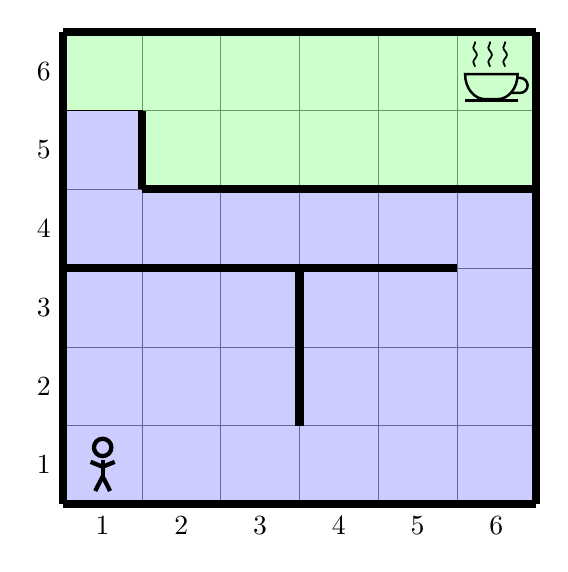
\begin{tikzpicture}
    % draw the grid and label the edges
    \draw[step=1cm,gray,very thin] (0,0) grid (6,6);
    \foreach \x in {1, ..., 6}
      \draw (\x cm - .5cm, 1pt) -- (\x cm - .5cm, -1pt)
      node[anchor=north] {$\x$};
      \foreach \y in {1, ..., 6}
      \draw (1pt,\y cm - .5cm) -- (-1pt, \y cm - .5cm)
      node[anchor=east] {$\y$};

      \draw[fill=green, fill opacity=.2] (0cm, 6cm) -- (6cm,6cm) --
      (6cm, 4cm) -- (1cm, 4cm) -- (1cm, 5cm) -- (0cm, 5cm) -- cycle;

      \draw[fill=blue, fill opacity=.2] (0cm, 5cm) -- (1cm, 5cm) --
      (1cm, 4cm) -- (6cm, 4cm) -- (6cm, 0cm) -- (0cm, 0cm) -- cycle;

      % add the agent and the goal
      \node (agent) at (.5cm, .5cm) {\Strichmaxerl[3]};
      \node (goal) at (5.5cm, 5.5cm) {\Coffeecup[3]};

      % Add some obstacles
      \draw[line width=3pt] (0cm, 3cm) -- (5cm, 3cm);
      \draw[line width=3pt] (3cm, 3cm) -- (3cm, 1cm);

      \draw[line width=3pt] (1cm, 4cm) -- (6cm, 4cm);
      \draw[line width=3pt] (1cm, 4cm) -- (1cm, 5cm);
  
      % border walls
      \draw[line width=3pt] (0cm, 0cm) -- (0cm, 6cm);
      \draw[line width=3pt] (0cm, 0cm) -- (6cm, 0cm);
      \draw[line width=3pt] (6cm, 6cm) -- (0cm, 6cm);
      \draw[line width=3pt] (6cm, 6cm) -- (6cm, 0cm);
  \end{tikzpicture}
  \caption{\label{fig:prob1_horizon_region1} MDP for problem 1c.}
\end{figure}
\FloatBarrier

\begin{enumerate}[a)]
\item Specify a reward function $R : S \times A \times S$ that will lead to the
  policy giving the shortest path to the coffee cup in states around
  the coffee cup. Try to keep the reward function as simple as possible.
\item Refer to Figure~\ref{fig:prob1_horizon_region1}. Using your
  reward function, Will the agent's policy in the green shaded region
  change compared to the MDP in Part~a? Justify your answer.
\item Refer to Figure~\ref{fig:prob1_horizon_region1}. Using your
  reward function, consider policy $\pi_a$ that in state $(1,5)$
  chooses action down, and a policy $\pi_b$ that in state
  $(1,5)$ chooses action up. How does $V_{\pi_a} ((1, 5))$ relate to
  $V_{\pi_b}((1,5))$?
\item Consider a policy $\pi_a$ and a policy $\pi_b$, where
  $\pi_a(s_{green}) = \pi_b(s_{green})$ and
  $\pi_a(s_{blue}) \not= \pi_b(s_{blue})$. How do $V_{\pi_a}$ relate
  to $V_{\pi_b}$? Explain.

\end{enumerate}

\section*{Problem 2}

In this problem you will program value iteration and policy
iteration. You will use environments implementing the OpenAI Gym
Environment API. For more information on the Gym and the API see:
\url{https://gym.openai.com/}. We will be working with different
versions of the FrozenLake
environment~\footnote{\url{https://gym.openai.com/envs/FrozenLake-v0}}.

In this domain the agent starts at a fixed starting position, marked
with ``S''. The agent can move up, down, left and right. In the
deterministic versions, the up action will always move the agent up,
the left will always move left, etc. In the stochastic versions, the
up action will move up with probability $1/3$, left with probability $1/3$
and right with probability $1/3$.

There are three different tile types: frozen, hole, and goal. When the
agent lands on a frozen tile it receives $0$ reward. When the agent
lands on a hole tile it receives $0$ reward and the episode ends. When
the agent lands on the goal tile it receives $+1$ reward and the episode
ends. We have provided you with two different maps.

States are represented as integers numbered from left to right, top to
bottom starting at zero. So the upper left corner of the 4x4 map is
state $0$, and the bottom right corner of the 4x4 map is state $15$.

You will implement value iteration and policy iteration using the
provided environments. You may use either Python 2.7 or Python 3. Some
function templates are provided for you to fill in. Specific coding
instructions are provided in the source code files.

\textbf{Note:} Be careful implementing value iteration and policy
evaluation. Keep in mind that in this environment the reward function
depends on the current state, the current action, and the \textbf{next
state}. Also terminal states are slightly different. Think about the
backup diagram for terminal states and how that will affect the
Bellman equation.

\subsection*{Coding (30 pt)}

Implement the functions in the code template. Then answer the questions below
using your implementation.

\subsection*{Part a (20 pt)}

Answer these questions for the maps
\texttt{Deterministic-4x4-FrozenLake-v0} and \\
\texttt{Deterministic-8x8-FrozenLake-v0}.

\begin{enumerate}[a)]
\item Using the environment, find the optimal policy using policy
  iteration. Record the time taken for execution, the number of policy
  improvement steps and the total number of policy evaluation
  steps. Use $\gamma=0.9$. Use a stopping tolerance of
  $10^{-3}$ for the policy evaluations.
\item What is the optimal policy for this map? Show as a grid of
  letters with ``U'', ``D'', ``L'', ``R'' representing the actions up,
  down, left, right respectively. See
  Figure~\ref{fig:prob2_example_policy} for an example of the expected
  output.  
\item Find the value function of this policy. Plot it as a color
  image, where each square shows its value as a color. See
  Figure~\ref{fig:prob3_value_image} for an example.
\item Find the optimal value function directly using value
  iteration. Record the time taken for execution, and the number of
  iterations required. Use $\gamma=0.9$ Use a stopping tolerance of
  $10^{-3}$.
\item Plot this value function as a color image, where each square
  shows its value as a color. See Figure~\ref{fig:prob3_value_image}
  for an example.
\item Which algorithm was faster? Which took less iterations?
\item Are there any differences in the value function?
\item Convert the optimal value function to the optimal policy. Show
  the policy a grid of letters with ``U'', ``D'', ``L'', ``R''
  representing the actions up, down, left, right respectively. See
  Figure~\ref{fig:prob2_example_policy} for an example of the expected
  output.
\item Write an agent that executes the optimal policy. Record the
  total cumulative discounted reward. Does this value match the value
  computed for the starting state? If not, explain why.
\end{enumerate}

\begin{figure}[ht]
  \centering
  \begin{BVerbatim}
LLLL
DDDD
UUUU
RRRR
  \end{BVerbatim}
  \caption{\label{fig:prob2_example_policy} Example policy for \texttt{FrozenLake-v0}}
\end{figure}

\begin{figure}[ht]
  \centering
  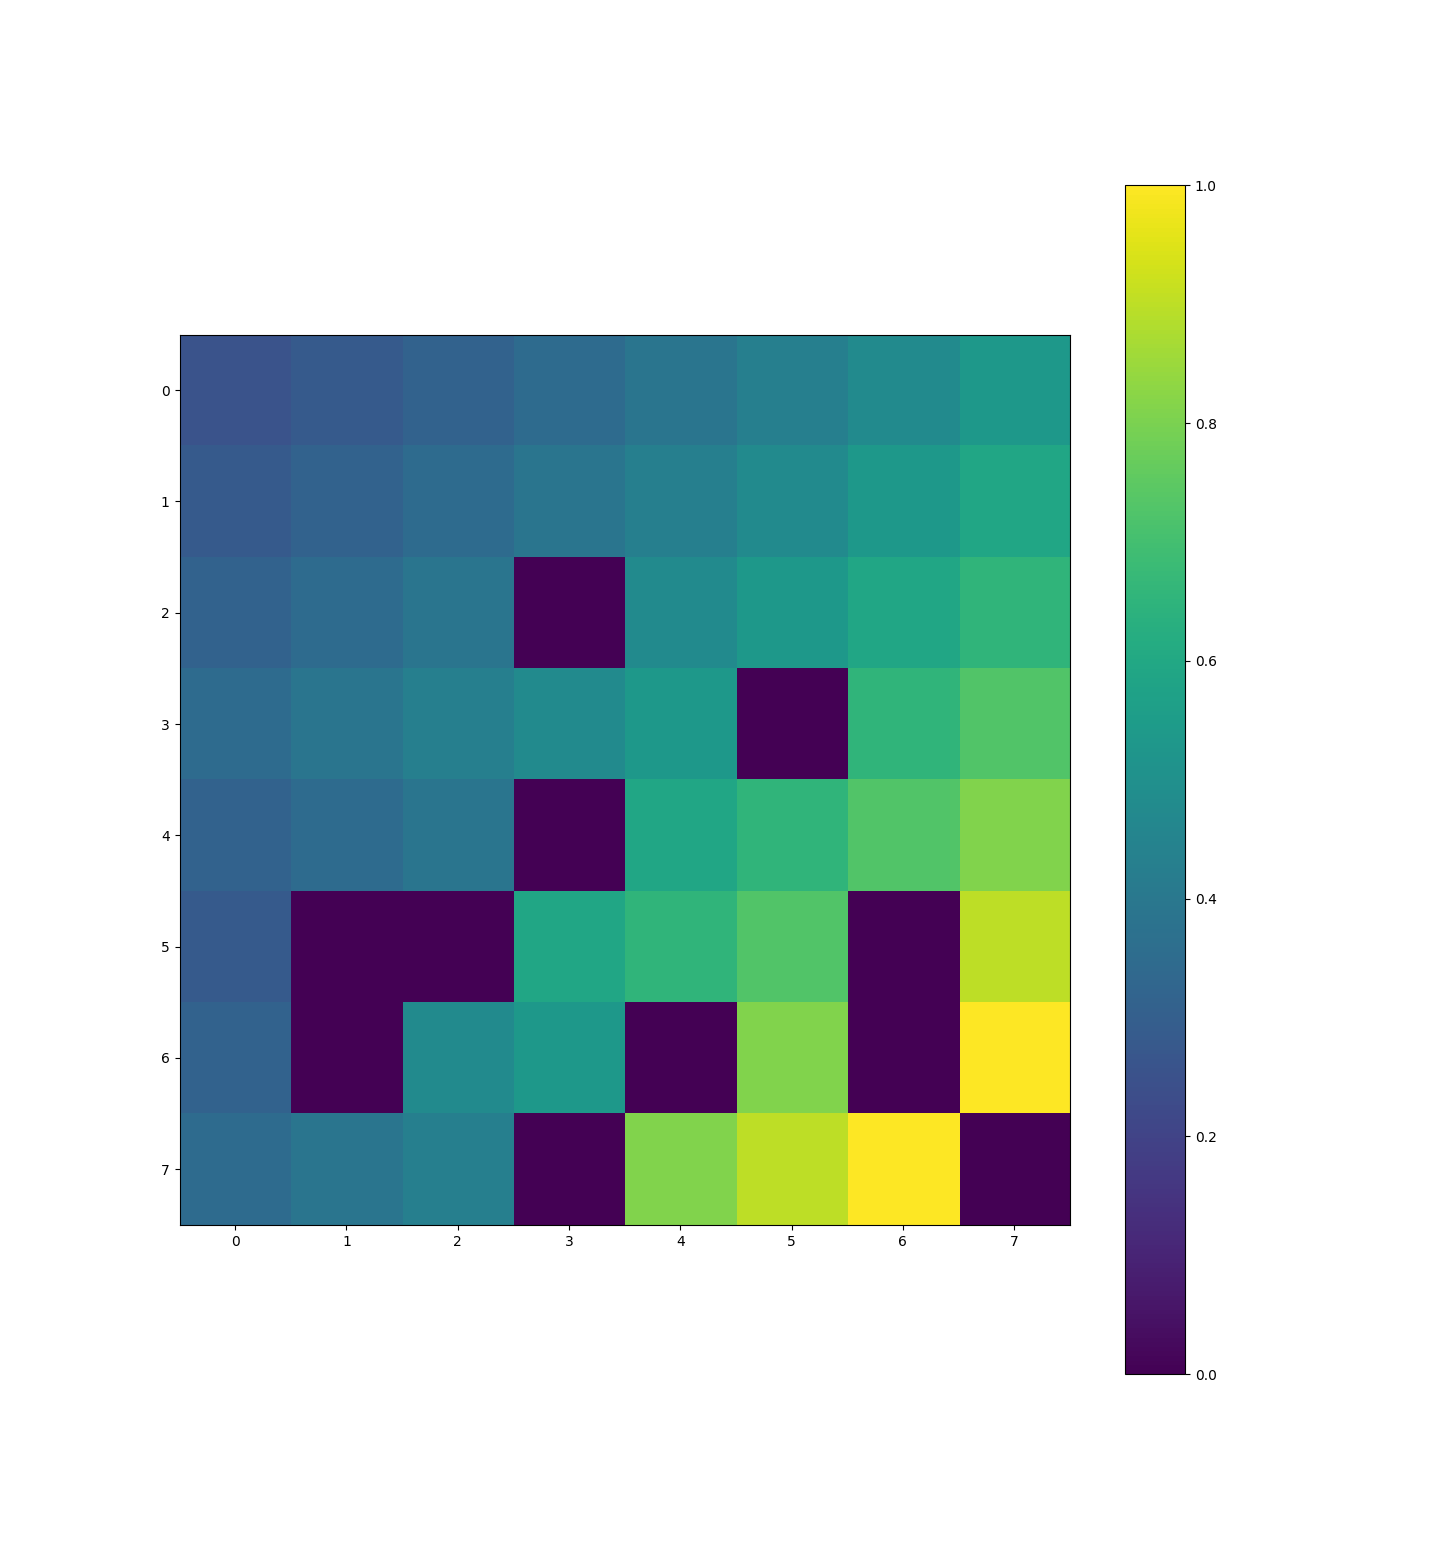
\includegraphics[width=.5\textwidth]{figures/value_function_plot.png}
  \caption{\label{fig:prob3_value_image} Example of value function
    color plot. Make sure you include the color bar or some kind of key.}
\end{figure}


\subsection*{Part b (10 pt)}

Answer the following questions for the maps
\texttt{Stochastic-4x4-FrozenLake-v0} and \\
\texttt{Stochastic-8x8-FrozenLake-v0}.

\begin{enumerate}[a)]
\item Using value iteration, find the optimal value function. Record
  the time taken for execution and the number of iterations required. Use a
  stopping tolerance of $10^{-3}$. Use $\gamma=0.9$.
\item Plot the value function as a color map like in Part~a. Is the
  value function different compared to the deterministic versions of
  the maps?
\item Convert this value function to the optimal policy and include it
  in the writeup.
\item Does the optimal policy differ from the optimal policy in the 
  deterministic map? 
  If so pick a state where the policy differs and explain why the action is
  different.
\item Write an agent that executes the optimal policy. Run this agent
  $100$ times on the map and record the total cumulative discounted
  reward. Average the results. Does this value match the value
  computed for the starting state? If not explain why.
\end{enumerate}

\subsection*{Part c (4 pt)}

We have provided one more version of the frozen lake environment. Now
the agent receives a $-1$ reward for landing on a frozen tile, $0$
reward for landing on a hole, and $+1$ for landing on the goal.

Answer these questions for map \texttt{Deterministic-4x4-neg-reward-FrozenLake-v0}.

\begin{enumerate}[a)]
\item Using value iteration, find the optimal value function. Use a
  stopping tolerance of $10^{-3}$. Use $\gamma=0.9$. Plot the
  value function as a color map like in Part~a.
\item Is the value function different from the other deterministic 4x4 map?
\item Convert the value function to the optimal policy and include it
  in the writeup.
\item Is the policy different from the other deterministic 4x4 map? If
  so, pick a state where it differs and explain why the action is different.
\end{enumerate}


\section*{Problem 3 (10pt)}

In this problem you will practice implementing an environment. Given
the following environment description implement an OpenAI Gym
environment that matches the specifications.

You have a server which contains three queues. Each queue can contain
up to five items. At every timestep the server is currently working on
a specific queue. The server starts the environment on queue 1. The
server has four actions: service an item from the current queue,
switch to queue 1, switch to queue 2, switch to queue 3. Servicing an
item from the queue when there is an item present gives a reward of
+1. When the queue is empty no reward is given. Switching queues gives
no rewards.

After each action each queue has a probability of receiving a new
item: $P1$, $P2$, and $P3$ for queue 1, 2, and 3 respectively.

Implement this environment with the following sets of probabilities:
  
\begin{itemize}
\item $P1 = 0.1$, $P2 = 0.9$, $P3 = 0.1$
\item $P1 = 0.1$, $P2 = 0.1$, $P3 = 0.1$
\end{itemize}

\section*{Problem 4 (10pt)}

Consider an MDP $M = (S, A, P, R, \gamma)$, where the components of 
$M$ are as described in Problem $1$. In this problem, we will study some properties
of value iteration. The Bellman optimality equation for the 
optimal value function $V ^* : S \to \mathbb R$, 
which we also write $V ^* \in \mathbb R ^S$, is
\begin{align*}
  V ^*(s) = \max _{a \in A} 
    \left(
      \sum _{s' \in S} 
        P(s' | s, a) \left(
          R (s, a, s') + \gamma V ^*( s' )
        \right)
    \right) .
\end{align*}
Define the Bellman optimality operator 
$\mathcal F ^* : \mathbb R ^{ S } \to \mathbb R ^{ S }$ as 
\begin{align*}
  \mathcal F ^* V (s) 
    = \max _{a \in A} 
      \left(
        \sum _{s' \in S} 
          P(s' | s, a) \left(
            R (s, a, s') + \gamma V ( s' )
          \right)
      \right) ,
\end{align*}
where $\mathcal F ^* V (s)$ is shorthand for $( \mathcal F ^* ( V ) ) (s)$.
Note that $S$ is finite so value functions are essentially vectors in 
$\mathbb R ^{ |S| }$. The operator $\mathcal F ^*$ maps vectors in 
$\mathbb R ^{ |S| }$ to vectors in $\mathbb R ^{ |S| }$.

Value iteration amounts to repeated application of $\mathcal F ^*$ to an 
arbitrary initial value function $V _0 \in \mathbb R ^ { S }$. 
\begin{enumerate}[a)]
  \item Prove that $V ^*$ is an unique fixed point of $\mathcal F ^*$, i.e, 
    $\mathcal F ^* V ^* = V ^*$ and that if 
    $\mathcal F ^* V = V$ and $\mathcal F ^* V ' = V '$ 
    for two value functions $V, V' \in \mathbb R ^S$, 
    then $V = V'$, i.e., $V(s) = V'(s)$ for all $s \in S$.
  \item Prove that $(\mathcal F ^*) ^ k V _0$ converges to $V ^*$ as $k \to \infty$
    for any $V _0 \in \mathbb R ^ S$. 
    Consider convergence in max-norm. The max-norm of a vector 
    $u \in \mathbb R ^d $ is defined as  
    ${ || u || } _\infty = \max _{i \in \{1, \ldots, d \} }{ | u _i | }$. 
  \item Given the optimal value function $V ^*$ 
    write down the expression that recovers the optimal policy $\pi ^*$ as a 
    function of $V ^*$ and the parameters of $M$.
    \footnote{Actually, such a procedure works for any value function $V \in \mathbb R ^S$. 
    This procedure is called policy extraction.}
\end{enumerate}

% some comments about what is important and is not important. 


\end{document}
